\section{\heiti 实验}

\subsection{\heiti 实验数据}


本实验采用开源的CAIL 2018数据集~\cite{xiao2018cail2018largescalelegaldataset}。该数据集包含1,927,685个案例,涵盖202种刑事罪名和183条刑法法规。其中,训练集有1,927,685条数据,测试集有216,829条数据。
为验证本文提出方法的有效性,本研究从CAIL 2018~\cite{xiao2018cail2018largescalelegaldataset}中按罪名分层采样10\%的数据,构建了CAIL Small数据集,用于消融实验和分析实验。CAIL Small和CAIL的数据分布如表~\ref{tab:cail}所示。
数据集中,多被告案件的法条分布常呈现长尾现象。如图\ref{fig:acc_dis}所示,各法条在判决结果中的出现频率及占比存在较大差异。在测试数据的法条分布中,占比最高的五种罪行是盗窃、危险驾驶、故意伤害和交通肇事,其占比分别为20.63\%、17.17\%、10.49\%、8.29\%和7.33\%。占比最高的十种罪行占总测试数据的73.58\%,而占比最少的100种罪行仅占总数据的1.83\%。
如图\ref{fig:art_dis}所示,法条数据分布同样呈现长尾趋势。占比最高的十种相关法条占测试数据的0.73\%,而占比最低的100种法条仅占2.44\%。

\begin{figure*}[!htbp]
	\begin{minipage}{0.5\linewidth}
		\centering
		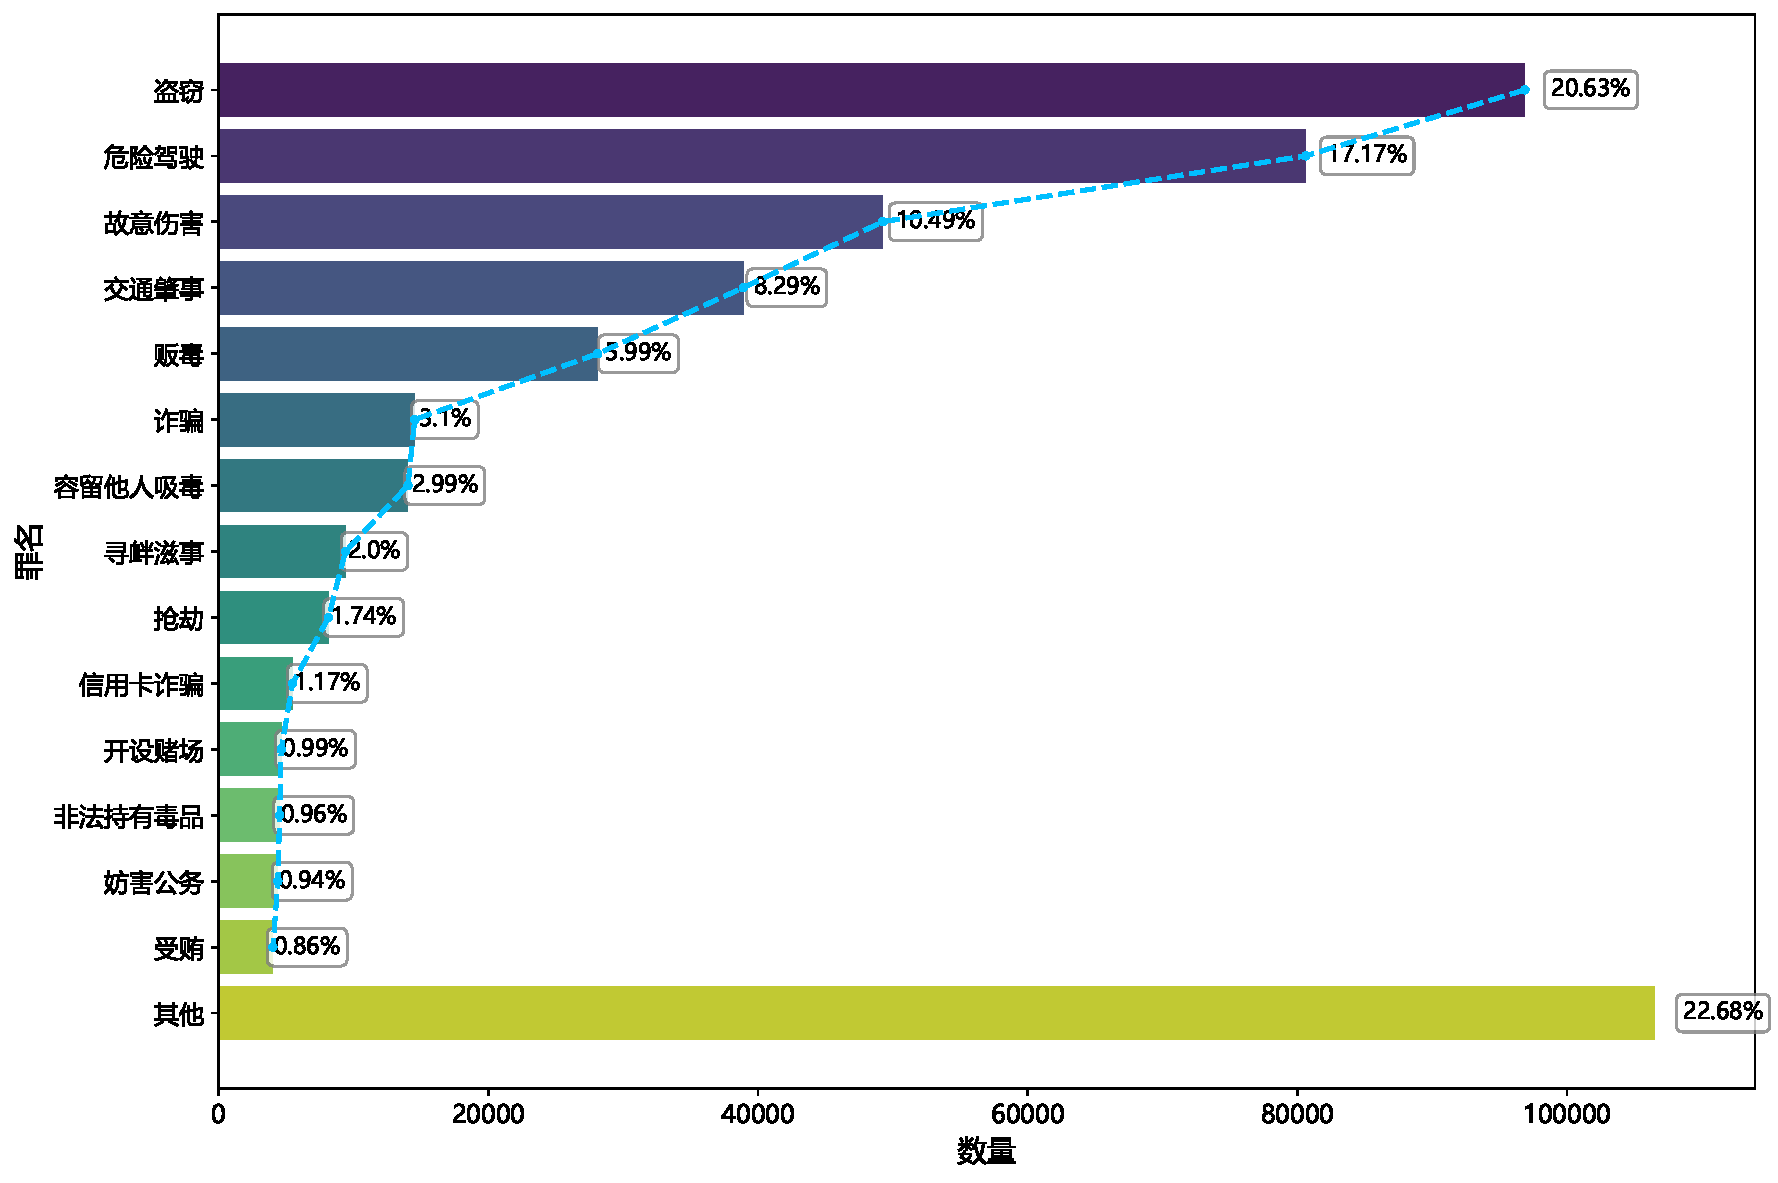
\includegraphics[width=1\linewidth]{fig/accusation_distribution.pdf}
		\caption{测试数据的罪名分布}
		\label{fig:art_dis}
	\end{minipage}
	\begin{minipage}{0.5\linewidth}
		\centering
		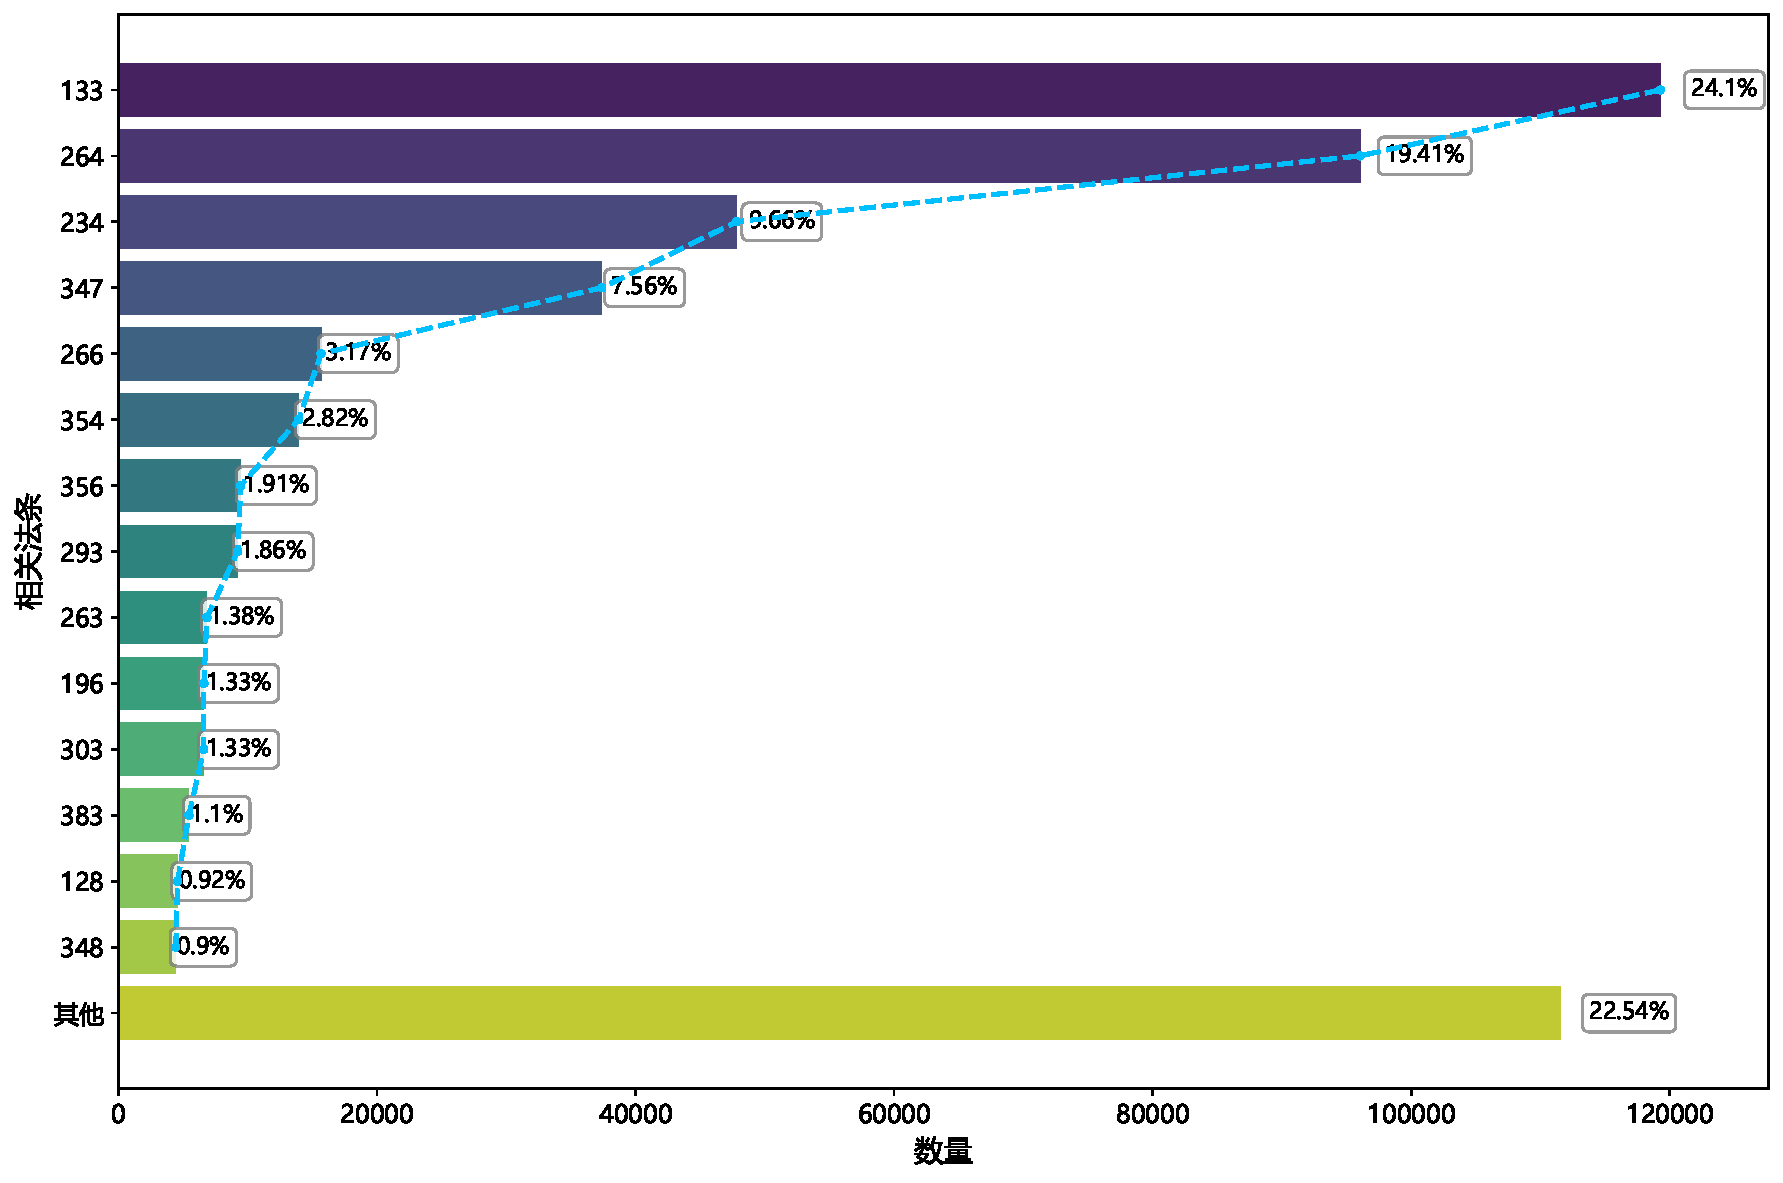
\includegraphics[width=1\linewidth]{fig/article_distribution.pdf}
		\caption{测试数据的法条数据分布}
		\label{fig:acc_dis}
	\end{minipage}
\end{figure*}
\subsection{\heiti 实验设置}
本研究利用CAIL 2018~\cite{xiao2018cail2018largescalelegaldataset}的训练集构建案例数据库。为在控制数据库规模的同时兼顾检索效率和案例代表性,本研究从训练集中每种罪名最多抽取100条数据,共构建1,676个案例。
法条数据库使用中国刑法典作为文本数据。
案例数据库和法条数据库的文本嵌入模型使用BAAI/BGE-m3模型~\cite{chenBGEM3EmbeddingMultiLingual2024}。
向量数据库采用Milvus~\cite{2022manu,2021milvus},相似度函数为内积(Inner Product, IP),向量索引方法为倒排索引(Inverted File, IVF),聚类中心设为200个。搜索算法采用暴力搜索(Flat Search),即在每个聚类内部使用相似度函数进行比较。要素提取模型采用Qwen-Turbo模型,判决模型使用Qwen-Plus模型~\cite{qwenQwen25TechnicalReport2025}。
CAIL 2018法律判决预测中的罪名和刑期预测两项子任务,均属于多标签多分类问题~\cite{xiao2018cail2018}。


\subsection{\heiti 评价指标}
本研究采用精确率(Precision, P)、召回率(Recall, R)和F1分数三项指标来衡量模型的预测效果。

\begin{equation}
	P=\frac{\sum_{i=1}^{n}TP_{i}}{\sum_{i=1}^{n}TP_{i}+\sum_{i=1}^{n}FP_{i}}
\end{equation}
\begin{equation}
	R=\frac{\sum_{i=1}^{n}TP_{i}}{\sum_{i=1}^{n}TP_{i}+\sum_{i=1}^{n}FN_{i}}
	\label{eq:recall}
\end{equation}
\begin{equation}
	F1=\frac{2\times P\times R}{P+R}
\end{equation}
其中,$i$为分类任务中类别的种类;$TP_i$为True Positive,指被正确地划分为类别 $i$ 的样本个数;$FP_i$ 为False Positive,指实际为其他类但被分类器划分为$i$ 类的样本数;$FN_i$ 为False Negative,指实际为 $i$ 类,但是被分类器划分错误的样本数。

\subsection{\heiti 基准模型}
为检验基座LLM的性能、本研究提出的“基于法条约束与类案融合的可解释司法判决预测方法”的有效性,以及其与基于域外语料训练的法律大模型相比的优劣,本研究在CAIL 2018数据集上进行了罪名和刑期两个子任务的对比实验,旨在比较本文模型与四种基线模型的性能差异。
基线模型包括基于词嵌入的深度学习模型MTL-Fusion~\cite{zhuopeng-etal-2020-multi}、中国司法长文本文书预训练模型Lawformer~\cite{xiao2021lawformer}、预训练模型BERT~\cite{fan2022multi},以及结合司法数据微调和RAG技术的LawChatGLM模型~\cite{JSJA202505027}。


\subsection{\heiti 实验结果与分析}

表\ref{tab:performance_comparison}的实验结果清晰揭示了不同技术路径在法律判决预测任务上的性能差异。从传统模型MTL-Fusion和Lawformer,到基于预训练的BERT,再到结合法律知识增强的LawChatGLM,模型在罪名和刑期预测上的性能呈现稳步提升趋势。这证明了更强的语义理解能力和外部知识引入是提升LJP性能的关键。然而,即使是表现最强的基准模型LawChatGLM,尽管通过检索法律条文提升了罪名预测的准确性,但在更需酌情裁量的刑期预测上仍有较大提升空间(F1分数为0.4691)。这表明仅依赖成文法条作为外部知识源尚不足以完全捕捉司法实践的复杂性。

\begin{table*}[htbp]
	\centering
	\begin{tabular}{lcccccc}
		\toprule
		\textbf{模型} & \multicolumn{3}{c}{\textbf{罪名}} & \multicolumn{3}{c}{\textbf{刑期}}                                                                        \\
		\cmidrule(lr){2-4} \cmidrule(lr){5-7}
		& \textbf{精确率}                    & \textbf{召回率}                    & \textbf{F1分数}   & \textbf{精确率}    & \textbf{召回率}   & \textbf{F1分数}   \\
		\midrule
		MTL-Fusion  & 0.6861                          & 0.6911                          & 0.6886          & 0.3512          & 0.3567         & 0.3539          \\
		Lawformer   & 0.6927                          & 0.7082                          & 0.7004          & 0.3581          & 0.3629         & 0.3605          \\
		BERT        & 0.7011                          & 0.7178                          & 0.7094          & 0.4311          & 0.4308         & 0.4309          \\
		LawChatGLM  & 0.7517                          & 0.7478                          & 0.7497          & 0.4712          & 0.4671         & 0.4691          \\
		Ours        & \textbf{0.7797}                 & \textbf{0.7689}                 & \textbf{0.7743} & \textbf{0.5578} & \textbf{0.566} & \textbf{0.5525} \\
		\bottomrule
	\end{tabular}
	\caption{ 法律判决预测结果的对比}
	\label{tab:performance_comparison}
\end{table*}

本文提出的方法在所有评价指标上均取得了最优表现,尤其在刑期预测任务上实现了关键突破,F1分数达到0.5525,相较于LawChatGLM提升了8.34\%。这一显著优势的核心原因在于我们创新的“法条约束与类案融合的可解释司法判决预测方法”。该框架不仅通过检索法律条文为罪名判定提供了权威的法律依据,更关键的是,通过引入“相似案例检索”模块,为模型提供了来自真实司法实践的量刑参考。这些相似判例中蕴含的裁判经验和量刑逻辑,有效弥补了成文法条在具体刑期裁量上的模糊性,使得模型的预测更贴近真实的司法裁判思维。实验结果有力证明,将LLM的推理能力与法律条文的规范性指引、相似案例的实践性参考进行深度融合,是构建高精度、高可靠性智能司法判决系统的有效路径。


\subsection{\heiti 消融实验}

\begin{table*}[!bp]
	\centering
	\begin{tabular}{cc|ccc|ccc|ccc}
		\hline
		\multicolumn{2}{c|}{\textbf{方法}} & \multicolumn{3}{|c|}{\textbf{罪名}} & \multicolumn{3}{|c|}{\textbf{刑期}} & \multicolumn{3}{|c}{\textbf{相关法条}}                                                                                                                \\
		\cline{1-2}\cline{3-5}\cline{6-8}\cline{9-11}
		\textbf{法条}                      & \textbf{类案}                       & \textbf{精确率}                      & \textbf{召回率}                       & \textbf{F1 分数} & \textbf{精确率} & \textbf{召回率} & \textbf{F1 分数} & \textbf{精确率} & \textbf{召回率} & \textbf{F1 分数} \\
		\hline
		$\checkmark$                     & $\checkmark$                      & 0.698                             & 0.669                              & 0.683          & 0.424        & 0.419        & 0.421          & 0.715        & 0.673        & 0.693          \\
		                                 & $\checkmark$                      & 0.697                             & 0.669                              & 0.683          & 0.424        & 0.414        & 0.418          & 0.634        & 0.615        & 0.624          \\
		$\checkmark$                     &                                   & 0.695                             & 0.671                              & 0.683          & 0.424        & 0.405        & 0.411          & 0.655        & 0.635        & 0.645          \\
		                                 &                                   & 0.684                             & 0.670                              & 0.677          & 0.364        & 0.387        & 0.349          & 0.634        & 0.615        & 0.624          \\
		\hline
	\end{tabular}
	\caption{消融实验}
	\label{tab:ablation}
\end{table*}
为验证本研究方法的有效性,我们对CAIL Small数据集的三个子任务进行了消融实验,结果如表~\ref{tab:ablation}所示。消融实验的重点在于评估法律条文检索模块和相似案例检索模块的作用,因此分别对这两个模块进行了实验。



\textbf{法律条文检索消融实验。}
为验证法律条文检索模块的有效性,我们在CAIL Small数据集中进行了消融实验。具体而言,在LLM进行多源信息融合推理时,我们移除了相关法律条文信息作为输入,但保留了三个相似案例作为参考。实验结果显示,在不使用法律条文信息后,相关法条预测的精确率下降了8.1\%,召回率下降了5.8\%,F1分数下降了6.9\%。此外,其他任务的性能也有一定程度的降低,这表明法律条文检索模块为LLM提供了重要的法律理论支持。


\textbf{相似案例检索消融实验。}
为验证相似案例检索模块的有效性,我们同样在CAIL Small数据集中进行了消融实验。具体而言,在LLM进行多源信息融合推理判决时,我们移除了相似案例库作为信息源,但保留了三个相关法律条文作为提示。根据表~\ref{tab:ablation}的结果,在不使用相似案例库后,刑期预测的F1分数下降了0.7\%,其余任务的性能也有所下降。这说明相似案例检索模块为LLM提供了关键的司法实践经验参考。


\subsection{\heiti 分析实验}
为确定最佳的相似案例检索和相关法条检索数量,我们在CAIL Small数据集上进行了分析实验。具体而言,我们对比了不同数量的相似案例和相关法条的Top-K参数对模型性能(F1分数)的影响。实验结果如图~\ref{fig:analysis}所示。

\begin{figure*}[htpb]
	\centering
	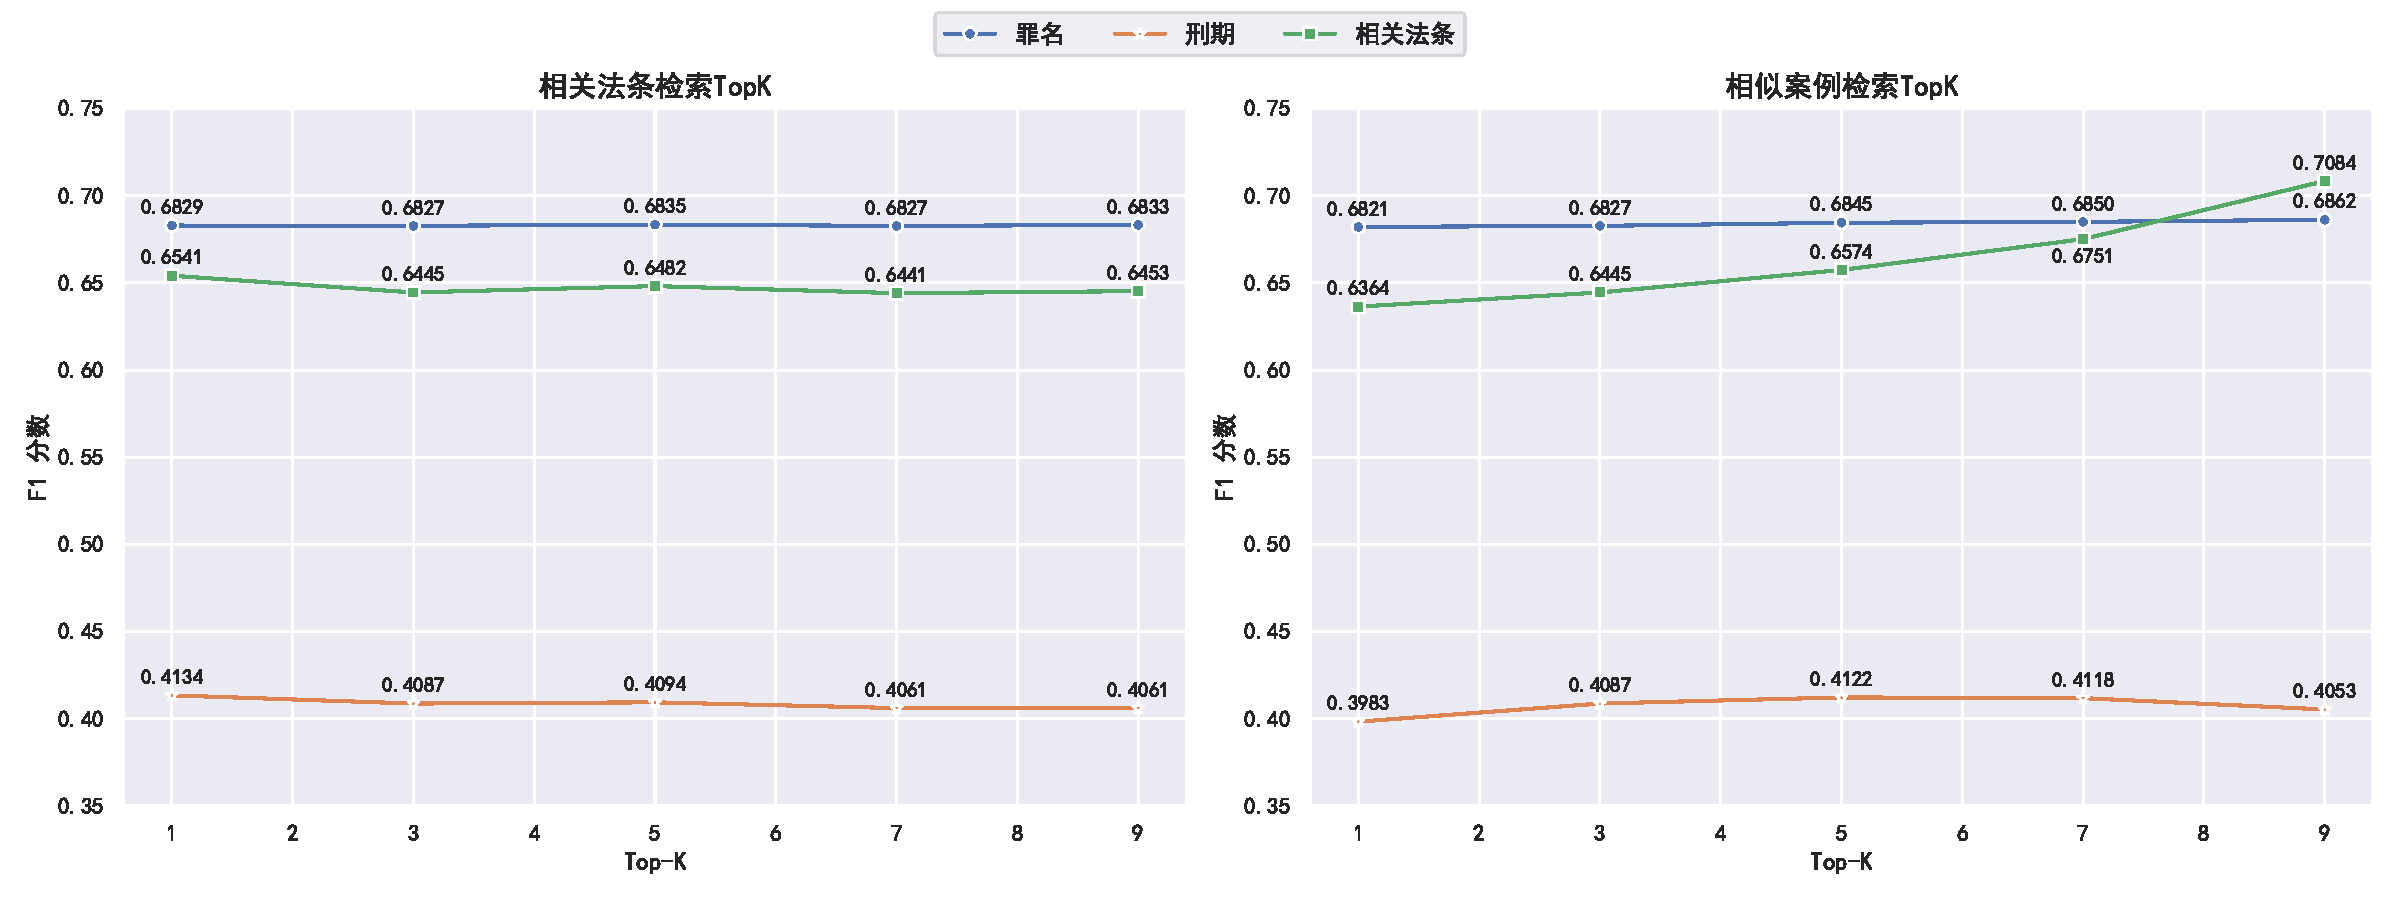
\includegraphics[width=0.8\linewidth]{fig/analysis.pdf}
	\caption{超参数TopK对模型性能的影响}
	\label{fig:analysis}
\end{figure*}

对于不同检索数量的相关法条,模型的整体F1分数在不同的Top-K值下保持稳定。这表明在检索相关法律条文时,模型的性能在此范围内对Top-K值不敏感。其原因在于法律条文通常明确且每个案件通常仅涉及一条或少数几条相关法条,因此即使Top-K值较小,相关法条检索也能提供足够的信息以进行准确判决。

对于不同数量的相似案例参考,模型在罪名预测和刑期预测上的F1分数相对稳定,但在相关法条预测上,F1分数随Top-K值的增加而逐渐提升。这表明在相似案例检索中,更多案例可提供更丰富的司法实践经验,从而提高模型的判决准确性。特别是对于法律定义边界模糊的罪名,更多的司法实践参考能帮助LLM更好地理解不同法律条文在实际应用中的区别,并更合理地应用法律条文。

\subsection{\heiti 案例研究}
\begin{figure*}[htpb]
	\centering
	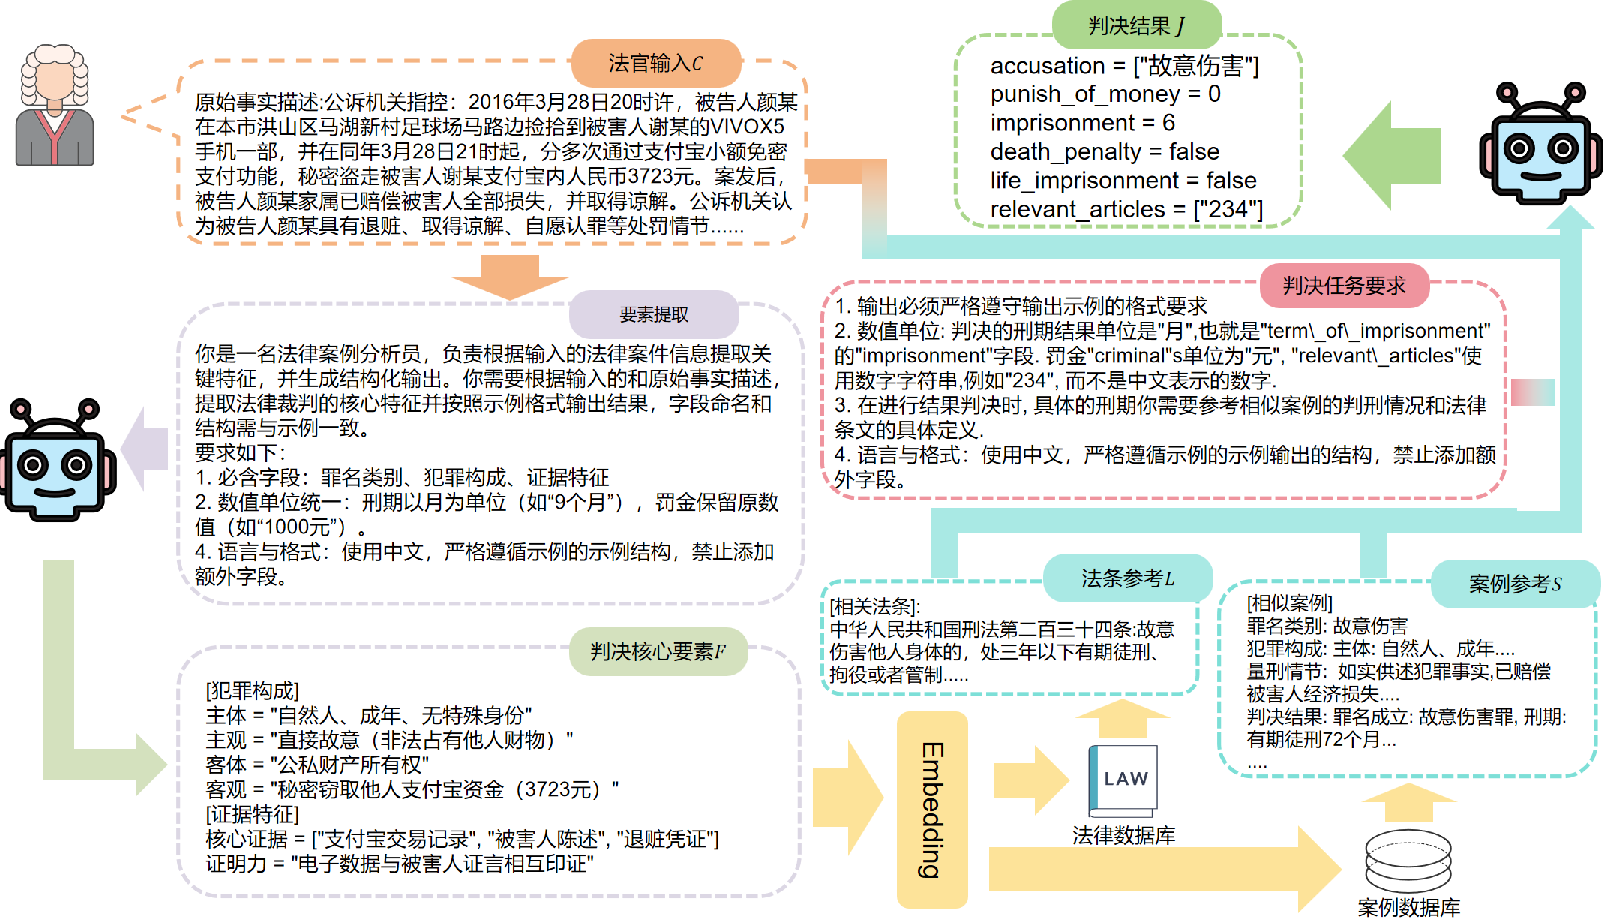
\includegraphics[width=0.8\linewidth]{fig/case.pdf}
	\caption{案例说明}
	\label{fig:case}
\end{figure*}
本研究提出的方法将以一个具体的盗窃案件为例进行说明。首先,系统接收一段原始的案件事实描述,例如:“公诉机关指控,2016年3月28日20时许,被告人颜某在…盗走被害人谢某支付宝内人民币3723元”。
接着,系统利用LLM对该文本进行“判决核心要素提取”,生成结构化的犯罪特征$F$:

\tbox{
主体 = "自然人、成年、无特殊身份"

主观 = "直接故意,非法占有他人财物"

客体 = "公私财产所有权"

客观 = "秘密窃取他人支付宝资金3723元"

核心证据 = ["支付宝交易记录", "被害人陈述", "退赃凭证"]

证明力 = "电子数据与被害人证言相互印证"
}

随后,进入本方法的核心——双重知识检索阶段。系统会将提取出的核心要素F通过文本嵌入模型BAAI/BGE-m3转换为高维查询向量。该查询向量被用于在两条并行路径上执行检索:第一条路径中,系统在预先向量化的法律数据库中进行近似最近邻(ANN)搜索,通过计算内积相似度,找出与案件特征最匹配的法律条文$L$:

\tbox{
中华人民共和国刑法第二百三十四条:故意伤害他人身体的,处三年以下有期徒刑、拘役或者管制.....
}

第二条路径中,系统同样利用该查询向量,在向量化的案例数据库中检索相似判例$S$:
\tbox{
罪名类别: 故意伤害;

犯罪构成:
\ \ \ \ 主体: 自然人、成年....;

\ \ \ \ 客体: 公私财产所有权;

量刑情节:如实供述犯罪事实,已赔偿被害人经济损失....;

判决结果:

\ \ \ \ 罪名成立: 故意伤害罪;

\ \ \ \ 刑期: 有期徒刑72个月...;
}
此处的案例检索更为精细,它会综合考量罪名、犯罪构成、证据特征等多个维度的相似度,以确保筛选出的历史判例与当前案件具有高度可比性。


最后,将原始案情($C$)、提取的核心要素$F$、检索到的法律条文$L$及相似案例$S$共同作为输入,送入核心LLM推理引擎,由其进行综合分析与推理,最终生成一个的结构化判决结果($J$):

\tbox{
accusation = ["盗窃罪"];

relevant\_articles = ["264"];

punish\_of\_money = 3723;

imprisonment = 7;

death\_penalty = false;

life\_imprisonment = false;
}